\chapter{Computational Spectral Unmixing}\label{chap:Csu}

\section{Introduction}

As discussed in \Cref{chap:Afssic}, spectral imaging is an important sensing technique that provides spectral information at each spatial location in the field-of-view, where often the end goal is spectral classification. However, the sensor is often part of a high-altitude platform such as an unmanned aerial vehicle (UAV) or satellite. In these remote sensing scenarios, the large standoff distances between the ground and the instrument result in large spatial resolutions. For example, in the Hyperion Imaging Spectrometer, which is satellite based, the spatial resolution is 30 meters \cite{folkman2001eo}. Due to the large spatial resolution, several materials are often measured together in the same pixel. This leads to a \gls{mixed spectrum} which consists of a combination of constituent spectra called \glspl{endmember}.

\begin{figure}[H]
	\centering
	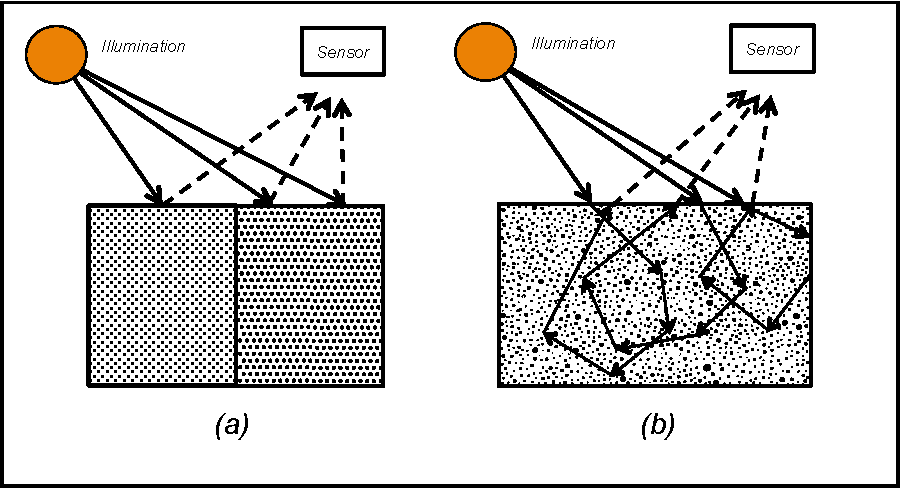
\includegraphics[scale=0.85]{linearAndNonlinearMixing.pdf}
	\captionof{figure}[Linear versus Non-Linear Mixing]{(a) Illustration of linear mixing where incident solar radiation reflects from a surface and the surface consists of distinct materials. (b) Illustration of nonlinear mixing where incident solar radiation encounters an intimate mixture of materials, reflecting multiple times before being reflected toward the spectral image sensor.}
	\label{fig:linearAndNonlinearMixing}
\end{figure}

\Gls{spectral unmixing} is the procedure by which the measured spectrum of a mixed pixel is decomposed into a set of \glspl{endmember} and a set of corresponding fractions called the \glspl{fractional abundance}. In this chapter, I will talk about my efforts to apply the techniques of computational sensing to directly estimate the \gls{fractional abundance} present in the \gls{mixed spectrum}. In the process, I will introduced a new computational spectral imaging architecture called the \gls{lcsi}. I will then provide simulation results that demonstate the advantage of spectral unmixing over traditional spectral imaging architectures which rely on point-by-point scanning techniques.

\section{Motivation}

There are two main reasons why mixed spectra occur \cite{keshava2002spectral, keshava2003survey}. First, if the spatial resolution of the sensor is low enough, separate materials can jointly occupy the \acrfull{fov} of a single pixel, the resulting spectral measurement is a combination of the spectra, see \Cref{fig:linearAndNonlinearMixing}(a). In this case, one can imagine the object scene as a \emph{checkerboard} mixture: light from the illumination source scatters or reflects from only one of the materials before being observed by the sensor, multiple scattering between materials are ignored. The second reason for mixed pixels occurs when different materials are combined into a homogeneous mixture, see \Cref{fig:linearAndNonlinearMixing}(b). In this case, mixed spectra are not caused by poor spatial resolution, they are inherent to the nature of the scene.

For the purposes of this chapter I will focus on the situation where mixed spectra arise due to the spatial resolution. Light from the illumination source scatters or reflects from only one of the materials before being observed by the sensor, we ignore multiple scattering between materials. 

If one is interested in quantifying how much of each material is present in the \gls{mixed spectrum} then spectral classification is not the preferred task. For example, in the \gls{afssi-c} we used the \acrfull{map} algorithm after each measurement step. The classification only reported on the most probable spectrum given the measurement data. Instead, \gls{spectral unmixing} should be used since the goal is to quantify how much of each \gls{endmember} is present in the \gls{mixed spectrum}. In this context, one refers to the spectral library as the endmember library, which is simply the set of possible spectra \cite{lillesand2014remote}. The relative amount of each of the constituent spectra is quantified by their respective \gls{fractional abundance}. 

When mixed spectra occur due to the spatial resolution limitation of the instrument, the fractional abundance is linearly proportional to the relative area of each material. This is called the linear mixing model \gls{lmm}, where the mixed spectrum can be written as 
%
\begin{equation}
\mb{f} = \sum_{r=1}^{N_{R}} x_r \mb{s}_r + \mb{e} = \mb{S} \mb{x}  + \mb{e}
\end{equation}
%
where $\mb{f}$ is the \gls{mixed spectrum}, $\mb{s}_r$ is the $r^{th}$ endmember spectrum, $\mb{S}$ is a matrix in which the columns are the endmember spectra, $\mb{x}$ is the fractional abundance vector, and $N_{R}$ is the number of endmembers in the endmember library. In the \gls{lmm}, the interactions amoung distinct endmembers are assumed to be neglible \cite{clark1984reflectance}. Each spectra has \gls{numspecchan} spectral channels.

There are two contraints imposed by the physics of the situation. Intuitively we should expect that the fractional abundance should be equal to or larger than zero. This is the \emph{nonnegativity} constraint:
%
\begin{equation}
	x_r \geq 0.
\end{equation}
%
We should also expect that if energy is conserved, i.e. there is no absorption of light, then the \gls{fractional abundance} should sum to one. This is he \emph{additivty} constraint:
%
\begin{equation}
	\sum_{r = 1}^{N_{\lambda}} x_r = 1
\end{equation}


\subsection{Unmixing in Traditional Spectral Imaging}

In traditional spectral imaging, the spectral datacube is first acquired by the instrument before any unmixing step is performed. Due to the nature of acquiring a 3-dimensional scene with a 1 or 2-dimensional \gls{fpa}, one often must resort to spatial or spectral scanning. Each measurement step only passes a fraction of the availible light emitted from the scene, constraining the \gls{snr}. As explained in \Cref{chap:Afssic}, this is often a time consuming process. 

The spectral datacube itself is contains a large amount of data. Significant attention has been focused on the computational burden induced by the high dimensionality of the data \cite{keshava2002spectral, keshava2003survey}. Prior to the unmixing step, the spectral datacube is first processing using a \gls{dimensionality reduction} step. This allows following computational steps to work with either a subset of the original data or to work in an alternative representation of the data which is used to significantly reduce the computational load.

If the spectral library is unknown, an \gls{endmember determination} step is used to estimate the spectra that constitute the mixed spectra. Finally the \gls{inversion} step is used to actually estimate the \gls{fractional abundance} of each mixed pixel in the spectral datacube. For the purposes of this chapter I will assume that the endmembers (spectral library) are known.


Dimensionality reduction and compression are similar but tend to have different goals. In dimensionality reduction, the goal is to find a smaller subset of data or an alternative representation to improve computational efficience and create an intuitive interpretation of the raw data. In data compression, the goal is to simply reduce the data so it can be more efficiently stored or transmitted, but in the end it will be decoded to approximate the original signal-of-interest's data. Since the spectral datacube is so large, especially in hyperspectral imaging, dimensionality reduction is almost always used as a pre-processing step. 

Data reduction algorithms are organized into two main types: statistical and non-statistical \cite{keshava2003survey}. Statistical algorithms include \acrfull{pca} and \acrfull{mnf}. As described in Chapter 2, \gls{pca} is applied to the measured  data in this case the spectal datacube and is used to find the bases with decorrelates the data by computing the eigenvectors of the data covariance matrix. In \gls{pca} there is typically observed that a steadily decreasing signal-to-noise ratio as the principal compenent number increases \cite{green1988transformation}. However, this is not always the case, because the procedure equates variance with information and is based on the assumption that the data structure can be described by a multi-dimensional normal distribution \cite{philpot2015mnf}. In \gls{mnf}, the algorithm attempts to order the components in terms of \gls{snr} which consists of two seperate \gls{pca} rotations and a noise whitening step. \gls{mnf} requires estimation of the noise covariance matrix in addition to the covariance of the data.

A non-statistical technique for dimensionality reduction is the optical real-time adaptive spectral identification system (ORASIS) \cite{bowles2007optical}, which is a series of steps that identify a subset of representative, or exemplar, pixels that convey the variables in a scene. When a new pixel is collects from the scene, a spectrum is compared to each examplar pixel using this angle metrix. If it is sufficently different then it is added to the set. Then using a modified Gram-Schmidt process, an orthogoal basis is created and a new dimension is added until the every exemplar can be represented well within a certain tolerances \cite{keshava2003survey}. 


Now I want to talk about inversion, this is the step that actually estimates the \gls{fractional abundance}. There are a variety of inversion techniques which actually attempt to estimate the fractional abundance vector. Many are based on minimizing the squared error and attempt to enforce additivity or non-negativity \cite{keshava2003survey, lawson1995solving}. A statistical non-parameteric technique attempts to minimize the variance of the estimator \cite{steven1993fundamentals}. There are also various algorithms based on \acrfull{map}, \acrfull{mle}, and clustering which can be used for spectral unmxing. Unfortunately, we cannot explore each inversion technique, due to there prevalence, I will use least-squares based inversion techniques when comparing computational spectral unmixing techniques. 


\section{Prior Efforts in Computational Spectral Unmixing}

In this chapter, I will discuss my efforts to apply the techniques of computational sensing to spectral unmixing. Computational sensing techiniques allows one to bypass the need to reconstruct the entire spectral datacube. By leveraging the Fellgett and Jacquinot advantage with sparsity promoting optimization algorithms, I show improved spectral unmixing performance. 


Several researchers have shown promising results in applying compressive sensing to spectral unmixing using a modified single-pixel camera architecture \cite{li2012compressive}. They demonstrated the ability to reconstruct the fractional abundance planes without the need to explicitly reconstruct the spectral datacube. In this approach, the object scene is imaged onto a \gls{dmd} and then a condensor lens focuses the reflected light into a whiskbroom spectrometer. One can think of this architecture as a set of parallel single-pixel cameras each operating at a different spectral channel, with the constraint that each \gls{dmd} must display the same pattern. This architecture does not code the spectral dimension of the spectral datacube. The researchers demonstrated compressive unmixing by minimizing the total variation (TV) of the endmember images. For example, in a normal computer monitor we typically have three endmembers images: the red image, the green image, and the blue image, which are combined to form the full color image. Thus the researchers minimized the total variation of the fractional abundance images while enforcing the nonnegativity constraint. 

In another effort, researchers use the \acrfull{cassi} architecture to perform compressive sensing on the spectral datacube and solve the $\ell_1$-regularized least squares problem (known as lasso in regression) to promote sparsity in the fractional abundances \cite{monsalve2015spectral}. Due to the nature of the single-disperser \gls{cassi} architecture, the researchs are forced to solve a larger joint-inference problem to preform spectral unmixing. 


\section{Architecture}

In my research I investigated the use of two architectures. The first architecture is the \gls{afssi-c} which was described in depth in \Cref{chap:Afssic}. The second architecture is a \acrfull{lcos} based spectral imager which allows for an extremely compact computational spectral imager called the \gls{lcsi}, which is shown in \Cref{fig:lcsiArchi}. The system provides a programmable wavelength dependent grayscale tranmission pattern, which can be independently addressed at each physical pixels of the \gls{slm}. The device is an array of micro cells of liquid crystal on a reflecting layer \cite{lazarev2012lcos}. Each layer of liquid crystal can be modeled as a thin retarder plate. Since most birefringent phase retarders are sensitive to wavelength, this element combined with a polarizing beam splitter or a linear polarizer produces a wavelength dependent transmission pattern, a spectral filter, which modulates the input spectra \cite{yuan2015compressive}.

\begin{figure}
	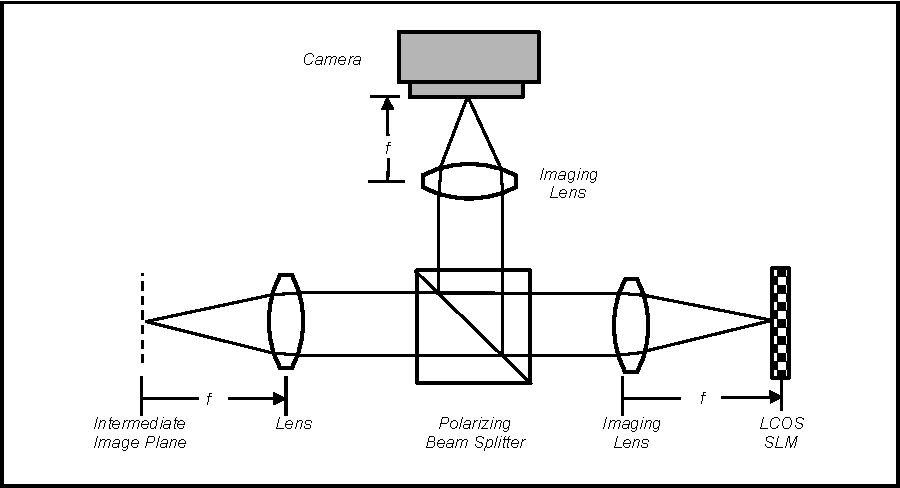
\includegraphics[scale=1.0]{lcsiArchi.pdf}
	\captionof{figure}[LCOS Based Spectral Imager]{The LCOS Spectral Imager. Light from the intermediate image plane is collimated. A polarizing beam splitter passes p-polarized light and rejects s-polarized light. Upon reflection of the LCOS SLM, the polarization state is changed to some elliptical polarization state. Only the s-polarized portion of the elliptical polarization is reflected toward the upper part where it is imaged onto a scientific camera. The intensity of the light that is passed depends on birefringence created by the programmable LCOS.}
	\label{fig:lcsiArchi}
\end{figure}

\subsection{How the LCOS Creates Spectral Filters}


Imagine an incident monochromatic plane wave traveling in the z-direction with a Jones polarization vector 
\begin{equation}
\mbh{a} = 
	\begin{bmatrix}
    	a_{x}  \\
    	a_{y} e^{ i \phi  }  \\
   \end{bmatrix}
\end{equation}
%
where $\phi$ is the phase differene between the x and y axes \cite{milster2013notes}. The full plane wave for the electric field can be written as

\begin{equation}
\mb{E} = A \exp \left[ \mb{k} \cdot \mb{r} - \omega t \right] \mbh{a}
\end{equation}
%
where there leading $A$ is a complex constant that adjusted for amplitude and absolute phase shift.
%
\begin{equation}
	\mb{k} = k \mbh{k} = k \ap{ \alpha \mbh{x} + \beta \mbh{y} + \gamma \mbh{z} }
\end{equation}
%
is the propagation vector with wavenumber $k = 2\pi /\ \lambda$ and direction cosines $\ap{\alpha, \beta, \gamma}$.

Transmitting through the polarizing beam splitter only passes horizontally polarized light

\begin{equation}
	\begin{bmatrix}
		a_x \\
		0 
	\end{bmatrix}
	=
	\begin{bmatrix}
		1 & 0 \\
		0 & 0
	\end{bmatrix}
	\begin{bmatrix}
		a_x  \\
		a_y e^{ i \phi  }
	\end{bmatrix}
	\label{eq:jonesAfterPBS1}
\end{equation}

The \gls{lcos} in our architecture is a phase only reflective type. Liquid crystal is used because it has the ability change birefringence $\Delta n$ when an electric field is applied. Birefringence is defined as 
%
\begin{equation}
	\Delta n = n_e - n_0
\end{equation}
%
where $n_0$ is the ordinary refractive index and $n_e$ is the extraordinary refractive index \cite{zhang2014fundamentals}. By changing the electric field in the cell the $\Delta n$ is changed. 

Birefringence is utilized to create retardation plates. These retardation plates serve to change the polarization state of input light. If one aligns the retardation plate so that the x polarized light is incident on the ordinary refractive index and the y polarized light is incident onto the ordinary refractive index then x and y polarizations are phase shifted by
%
\begin{equation}
	\eta = \frac{2 \pi}{\lambda} \left[ n_e\ap{\lambda} - n_o \ap{\lambda} \right] T
\end{equation}
%
where $T$ is the physical thickness of the plate, where the $ n_e \ap{ \lambda } $ and $ n_o \ap{\lambda} $ are index of refraction of the extraordinary and ordinary waves which are wavelength dependant functions \cite{milster2013notes}. 

%The general Jones matrix for an arbitrary birefringent material as a retardation plate is
%
%\begin{equation}
%	\begin{bmatrix}
%		M_{11} & M_{12} \\
%		M_{21} & M_{22}
% 	\end{bmatrix}
% 	=
% 	\begin{bmatrix}
% 		e^{i \eta/2} \cos^2 \theta + e^{-i \eta/2} \sin^2 \theta & \ap{ e^{i \eta/2} - e^{-i \eta/2} } e^{-i \phi} \cos \theta \sin \theta \\
% 		\ap{ e^{i \eta/2} - e^{-i \eta/2} } e^{i \phi} \cos \theta \sin \theta & e^{i \eta/2} \sin^2 \theta + e^{-i \eta/2} \cos^2 \theta
% 	\end{bmatrix}
% 	\label{eq:arbJonesMatrix}
% \end{equation}
% %
% where the relative phase retardation between the fast and slow axes is given by $\eta = \phi_y - \phi_x$, $\theta$ is the orientation of the fast axis with respect to the x-axis, and $\phi$ is the circularity. Thus after propagating from the LCOS the Jones Vector is written as
% %
% \begin{equation}
% 	\begin{bmatrix}
% 		a_x M_{11} \\
% 		a_x M_{21}
% 	\end{bmatrix}	
% \end{equation}
% %
% finally the vertical polarization (y) is reflected by the polarizing beam splitter towards the camera
% %
% \begin{equation}
% 	\begin{bmatrix}
% 		0 \\
% 		a_x M_{21}
% 	\end{bmatrix}	
% \end{equation}

% Where the intensity is pro



% The phase shift can be used to change the polarization state of the light. For example, when linearly polarized light at 45 degrees goes through a phase shift of $\Delta = \lambda / 2$ the polarized light will rotate to vertical. However, this is a special case and in general the output light will be elliptically polarized. When elliptically polarized light is incident onto a linear polarizer, only linearly polarized light is passed, the intensity of the light passed however depends on the relative amplitude and phase of the x and y polarizations of the incident light \cite{milster2013notes}. 

Unfortunately, a full discussion of polarization is out of the context of this disseration. The important point is that for light of a single wavelength, the \gls{lcos} can manipulate the polarization, which in general is not linearly polarized. Placing a polarizer after light has been reflected from the \gls{lcos} will force the transmitted light to be linearly polarized but at an intensity depedent on the projection of the input polarization. The ordinary and extraordinary index of refraction depdend on the wavelength of light. Thus phase shift imparted to the two polarizations will be wavelength depdent. Passing non-monochromatic light to an \gls{lcos} and then a linear polarizer will impart a wavelength depdent intensity. In short, the \gls{slm} provides polarization and wavelength depdent transmission patterns to encoded the spectral datacube \cite{tsai2015spatial}.


\subsection{Forward Model}

The forward model for the LCOS spectral imager is similar to the one presented in \Cref{ssec:afssicForwardModel}. Except now we do not have to account for dispersion when imaging from the input plane to the LCOS and from the LCOS to the \gls{fpa} of the camera. I will thus skip the derivation of the forward model and simply present the final equation for the measurement value at pixel $n$ and $l$ from the camera:
%
\begin{align} 
	\Gamma_{nl} &= \sum_{n^\prime l^\prime} \iiint \mbox{rect} \left( \frac{x}{\Delta} - l, \frac{y}{\Delta} - n \right) \mbox{rect} \left( \frac{x}{\Delta} - l^\prime , \frac{y}{\Delta} - n^\prime \right) \notag \\
 	&\qquad \times T_{n^\prime l^\prime} D_0 \left( x, y; \lambda \right) dx \, dy \, d\lambda.
\end{align}
%
Notice that there is no dispersion constraint that we encounted in the \gls{afssi-c} or a joint spatial-spectral contraints like in the \gls{cassi}. If one so choose to, one can simply treat each pixel in the image as completely indepdent from neighboring pixels. This greatly simplifies the analysis. 

Similar to the \gls{afssi-c} we can further simplify this by imagining a discrete spectral density, the spectral datacube. The discretized source spectral datacube is $D_{nlc}$, and then the detector signal $\Gamma_{nl}$ is a result of spectral filter created by the PBS-LCOS combination $T$ acting on the pixelated source is
%
%
\begin{equation}
	\Gamma_{n,l} = \sum^{N_{\lambda}-1}_{c = 0} T_{n,l,c} D_{n,l,c} \,
\end{equation}
%
%
which shows the measurement at each pixel being the inner product of the source spectrum and the spectral filter which results from the spectral filter created by the PBS-LCOS combination. In a single spatial location, this reduces to a simple inner product
%
\begin{equation}
	g_m = \mb{h}_m^{T} \mb{f} 
\end{equation}
%
where the subscript $m$ represents the $m^{\text{th}}$ measurement step and $\mb{f}$ the true spectrum at that pixel. Notice that this forward model is does not exhibit any dispersion constraint like the one in the \gls{afssi-c}. For a sequence of measurements this simplies to 
%
\begin{equation}
	\mb{g} = \mb{H} \mb{f}
\end{equation}
%
where the rows of $\mb{H}$ is $\mb{h}_m^T$ and $\mb{g}$ is an $m \times$ 1 vector. However, the spectral $\mb{f}$ is a mixed spectrum

\begin{equation}
	\mb{f} = \mb{S}\mb{x}
\end{equation}
%
Thus for a sequence of noisy measurements at a single pixel
%
\begin{equation}
	\mb{g} = \mb{H}\mb{S}\mb{x} + \mb{e} = \mb{A}\mb{x} + \mb{e}
\end{equation}\label{eq:csuForwardModel}
%
where $\mb{H}$ is an $N_m \times N_{\lambda}$ matrix, $\mb{S}$ is the endmember library which is an $N_{\lambda} \times N_{R}$ matrix, $\mb{x}$ is the fractional abundance vector which an $N_R \times 1$ vector, $\mb{e}$ is the additive noise which is a $N_m \times 1$ vector. I define $\mb{A} = \mb{H} \mb{S}$. In this context, we can think of $\mb{H}$ as the sensing matrix and $\mb{S}$ as the representation matrix as discussed in \Cref{sec:compressiveSesing}.

\section{Prior work using LCOS Computational Spectral Imaging}

Several computational spectral imaging results have already utilized variations of liquid crystal technology for computational spectral imaging. The first instance, in 2012, demonstrated a single-pixel liquid crystal device to demonstrate compressive spectroscopy and exhibited a 10$\times$ reduction in the number of measurements compared to a traditional ismorphic spectrometer \cite{august2013compressive}. Shortly after in 2013, a demonstration of a compressive spectral imager using an \gls{lcos} \gls{slm} was published which jointly coded spatial and spectral features for \cite{zhu2013coded}. In 2015, a  hyperspectral imaging sensor demonstrated which used the \gls{lcos} \gls{slm} to perform blind compressive sensing. This architecture uses a Bayesian approach to learning the dictionary (basically a respresentation basis) \emph{in situ}. This experiment incorporated side-information from a conventional color camera to perform spectral datacube reconstruction \cite{yuan2015compressive}. That same year, a miniture ultraspectral imaging system based on a custom built liquid crystal cell, which applies the same spectral filter to each spatial location, demonstrated the ability to reconstruction gigapixel spectral datacubes with less than an order of magnitude measuremesure required by conventional systems \cite{august2016miniature}. 


\section{Solving the Inverse Problem}

In the \gls{afssi-c} and in the LCOS Spectral Imager, measurements are acquired in a time sequential manner. A traditional isomorphic spectral imager which uses a tunable filter also acquires measurements in a time sequential manner. In this setup the rows of $\mb{H}$ are the spectral filters which have more than one nonzero element for the \gls{afssi-c} and LCOS spectral imager. While in the tunable filter $\mb{H} = \mb{I}$ which is an $N_{\lambda} \times N_{\lambda}$ identity matrix, so each row has only one non-zero element.  In all three architectures the inverse problem is: given $\mb{H}$, $\mb{S}$, $\mb{g}$ estimate the fractional abundance $\mbh{x}$ after m number of measurement steps.


In all three architectures, in general one is faced with underdetermined or overdetermined systems of equations $N_m \neq N_{R}$. One of the common inversion techniques is the least-squares estimator (LSE) \cite{keshava2003survey} which is derived in Appendix \ref{app:Derivation of the Least Squares Estimator}. In this context the closed form unconstrained LSE is
%
\begin{equation}
	\mbh{x} = \ap{ \mb{A}^T \mb{A} }^{-1} \mb{A}^T \mb{g}
\end{equation}
%
which by definition attempts to minimize the square error between the observed data and the forward model. Various constraints can be imposed such as additivity and nonnegativity. 

As I mentioned earlier, remote sensing the fractional abundance vector $\mbh{x}$ tends to be sparse. This is because number of endmembers in the library is much larger than number of endmembers that are actually present in the mixed spectrum $N_{R} > \| \mb{x} \|_0$. Therefore, we can begin to invoke some of the concepts of compressive sensing such as minimizing the $\ell_1$ regularized least-squares objective function to find solutions that are sparse:

%
\begin{equation}
	\mbh{x} = \argminA_{\mb{x}} \: \| \mb{Ax} - \mb{g} \|_{2}^{2} + \tau \| \mb{x} \|_1
	\label{eq:l1reglsV2}
\end{equation}
%
For my simulations and experiments I have chosen to use the built-in MATLAB \texttt{lasso} function. 

\section{Results}

I next propose codes for both the \gls{afssi-c} and LCOS spectral imaging architecture. 

In the \gls{afssi-c} architecture one is restricted to producing binary codes $ \{ -1, +1 \}$ codes using the \gls{dmd}. We can thus choose to measure spectral channels one at time, i.e. turn on one mirror per measurement step. This is the same thing as a tunable filter approach. Where the measurement matrix is equal to the identity matrix $\mb{H} = \mb{I}$.
Combining the tunable filter approach with the LSE produces what one should expect from a traditional isomorphic spectral imager to conduct spectral unmixing.

We can also use random binary codes to achieve a multiplexed measurement. As demonstrated both the \gls{scout} and the \gls{afssi-c}, we expect that sampling multiple spectral channels per measurement should improve the unmixing error. 

The error metric used to measure the unmixing error is the \acrfull{rmse} between the estimated fractional abundance $\mbh{a}$ and the ground truth fractional abundance $\mb{a}$

\begin{equation}
	RMSE =  \left[ \frac{1}{N_R} \sum_{r = 1}^{N_{R}} \ap{ \hat{a}_r - a_r }^2 \right]^{\frac{1}{2}}
\end{equation}

\subsection{Adaptive Unmixing Algorithm For the AFSSI-C}

We developed an adaptive unmixing algorithm for creating spectral filters is which similar to the one used for creating spectral filters in spectral classification. The basic idea is that a modified version of \gls{pca} is used to create adaptive spectral filters. This algorithm begins with the spectral library which consist of the endmember spectra $\mb{S}$. Initially, before any measurements are made, the estimated fractional abundances of each endmember are the same 
%
\begin{equation}
	\mbh{a}_{m=0} = \frac{1}{N_R} \mb{1}
\end{equation}
%
where $\mb{1} \in \mathbb{R}^{N_R}$where the subscript $m$ denotes the measurement step, $m=0$ is before any measurement has been recorded. The each endmember in the spectral library is then weighted by the square of their respective estimated fractional abundance
%
\begin{equation}
	\mb{S}_w = 
	\begin{bmatrix}
		\hat{a}_1^2 \mb{s}_1 & \hat{a}_2^2 \mb{s}_2 & \hdots & \hat{a}_{N_R}^2 \mb{s}_{N_R}
	\end{bmatrix}
	\label{eq:weightedSpectralLibrary}
\end{equation}

Then the eigenvectors of the unnormalized covariance matrix of the weighted spectral library are computed. 
%
\begin{equation}
	X_m = \mb{S}_w \mb{S}_w^T 
\end{equation}
%
These are the principal component vectors. Where the first principal component corresponds to the direction of largest variance and so on. Initially, for the first measurement, the algorithm chooses the first principal component for the spectral filter $\mb{h}_{m=1} = \mb{p}_1$. The measurement is then recorded
%
\begin{equation}
g_m = \mb{h}_{m}^{T} \mb{f} + e_m
\end{equation}
%
where $\mb{S}$ is NOT the weighted spectral library matrix, it is the the regular spectral library. After the measurement is recorded, the $\ell_2$ norm of the difference between the guess measurement and the actual measurement is recorded:
%
\begin{equation}
	\xi_m = \| \mb{h}_{m}^{T} \mb{S} \mbh{a}_{m-1} - g_m \|_2 
\end{equation}
%
notice that the guess measurement $\mb{h}_{m}^{T} \mb{S} \mbh{a}_{m-1}$ is the measurement we would expect in the case of no noise and with the estimated fractional abundance from the previous measurement. 

The fractional abundance is then estimated. In practice, least-squares estimator is used for the first measurement step. After the first measurement, the MATLAB \texttt{lasso} is used. This is because the function requires atleast two rows or entries to run. The spectral library is then weighted again through \Cref{eq:weightedSpectralLibrary}. Again the principal components are recomputed, and for the second spectral filter, the algorithm uses the second principal component from the covariance of the newly reweighted spectral library. After the measurement has been recorded, the  $\ell_2$ norm of the difference between the guess measurement and the actual measurement is computed again $\xi_m$. Again the weighted spectral library is recomputed as well as the principal components. 

If the $\xi_m > \xi_{m-1} - {\sigma}/{2}$ then the next principal component is used for the next spectral filter. Otherwise the first principal component is used again.  We constrain the algorithm to only use the first six principal components, this is because we noticed that the unmixing preformance is optimized when limited to only the first six principal components. Intuitively, this occurs because higher principal components tend be higher frequency where noise begins to dominate the signal and the spectra generated by our sources tend to be lower frequency. In short, if the difference between the guess measurement and the actual measurement is improving, the algorithm continues to select the next principal component from the weighted spectral library library. If the difference has not changed then, the algorithm goes back to the first principal component. This algorithm is called the switching \gls{swpca}. The algorithm and MATLAB code is posted in Appendix BLAH BLAH BLAH. 




\section{Results}




